\newcommand{\PaperWallet}{
 \begin{tikzpicture}[framed,inner frame sep=0]
  \node[coordinate] at (0pt,0pt) (topleft) {};
  \node[anchor=north west,inner sep=0pt] at (topleft) {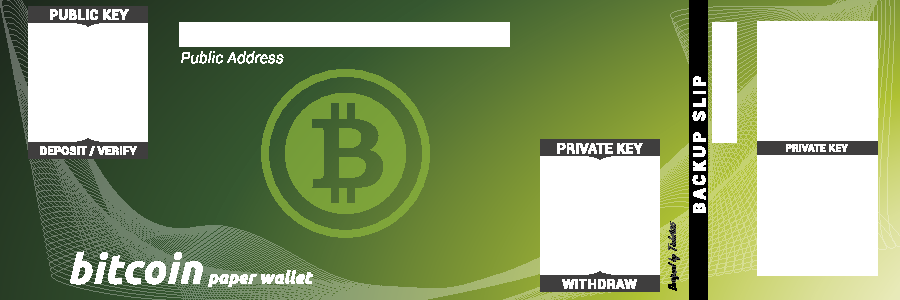
\includegraphics[width=180mm]{notes/note_Timbo925_Green.pdf}};
  \node[anchor=center,inner sep=0] at ($(topleft)+(6.1mm,-28.4mm)+(12mm,12mm)$) (QRCode1) {
   \resizebox{22mm}{!}{%
    \begin{pspicture}(50mm,50mm)
     \psbarcode[linecolor=black!80!white]{\insertAddress}{eclevel=H}{qrcode}
    \end{pspicture}}};
  \node[anchor=center,inner sep=0,rotate=90] at ($(topleft)+(151.5mm,-28.5mm)+(12mm,12mm)$) (QRCode1) {
   \resizebox{22mm}{!}{%
    \begin{pspicture}(50mm,50mm)
     \psbarcode[linecolor=black!80!white]{\insertAddress}{eclevel=H}{qrcode}
    \end{pspicture}}};
  \node[anchor=center,inner sep=0] at ($(topleft)+(108.0mm,-55.2mm)+(12mm,12mm)$) (QRCode2) {
   \resizebox{22mm}{!}{%
    \begin{pspicture}(50mm,50mm)
     \psbarcode[linecolor=red!60!black]{\insertPrivKey}{eclevel=H}{qrcode}
    \end{pspicture}}};
  \node[anchor=center,inner sep=0,rotate=90] at ($(topleft)+(151.5mm,-55.2mm)+(12mm,12mm)$) (QRCode2) {
   \resizebox{22mm}{!}{%
    \begin{pspicture}(50mm,50mm)
     \psbarcode[linecolor=red!60!black]{\insertPrivKey}{eclevel=H}{qrcode}
    \end{pspicture}}};
  \node[anchor=west,font=\small\bfseries] at ($(topleft)+(36mm,-7mm)$) (Address) {\insertAddress};
  \node[anchor=west,font=\small\bfseries,rotate=90] at ($(topleft)+(145mm,-28.7mm)$) (Address2) {\expandafter\substr\expandafter{\insertAddress}{1}{12}};
 \end{tikzpicture}
}
